%----------------------------------------------------------------------------------------
\chapter{Contribution} % possible chapter for Projects
\label{chap:contribution}

\section{Introduction to the Fair-by-Design Workflow}
\label{section:workflow-introduction}

In recent years, the heightened scrutiny of the ethical implications associated with artificial intelligence (AI) and machine learning (ML) systems has emerged as a response to the escalating influence of these technologies, particularly in domains where consequential decisions profoundly impact individuals' lives. The evolving landscape of AI ethics necessitates a conscientious examination of the ethical dimensions embedded in the development and deployment of these systems.

Within this multifaceted ethical discourse, the imperative of integrating fairness into the fabric of AI design has emerged as a paramount consideration. The principle of fairness, when applied as a foundational element in the design process, underscores the need for AI systems to produce outcomes that are not only accurate and efficient but also just and equitable. Achieving fairness in AI development demands a comprehensive and deliberate approach, one that transcends mere post hoc considerations by embedding fairness principles from the very inception of the design process.

The conceptual framework of a fair-by-design workflow encapsulates a meticulous set of principles and procedural steps, each strategically devised to ensure the attainment of equitable and unbiased outcomes throughout the entire lifecycle of an AI system. This includes not only the initial design and development phases but also extends to the implementation, deployment, and ongoing monitoring stages. The iterative nature of this workflow acknowledges the dynamic interplay between ethical considerations and technological advancements, emphasizing the continuous reassessment and refinement of fairness strategies.

By adopting a fair-by-design approach, stakeholders in AI development, ranging from researchers and engineers to policymakers and end-users, commit to a shared responsibility for cultivating a technological landscape where the ethical imperatives of fairness and equity are not afterthoughts but integral components steering the trajectory of AI systems towards societal benefit and justice. In essence, the pursuit of ethical AI underscores not only the advancement of technological capabilities but also the conscientious stewardship of these capabilities to ensure they align with ethical norms and societal values.

\subsection{Principles of Fair-by-Design Workflow}
\label{subsection:workflow-principles}

\begin{enumerate}

    \item \emph{Proactive Fairness Integration:} The cornerstone of the Fair-by-Design workflow lies in the proactive embedding of fairness considerations at the genesis of the design process, diverging from conventional practices where fairness is often retroactively addressed after system implementation. This proactive approach marks a transformative shift in the landscape of algorithmic development, underscoring the ethical imperative of forethought in anticipating and mitigating biases. Seamless integration of fairness into the initial design stages aims to forestall the emergence of discriminatory outcomes, establishing a bedrock rooted in equitable principles. Beyond its alignment with ethical standards, this proactive integration streamlines the developmental trajectory, fostering a more responsible and inclusive machine learning environment. This meticulous attention to fairness from the inception reflects a commitment to ethical AI practices that transcend mere compliance, embodying a conscientious endeavor to uphold societal values and ensure the equitable treatment of diverse individuals impacted by AI systems.

    \item \emph{Transparency and Explainability:} The Fair-by-Design workflow places a premium on transparent documentation of design decisions and algorithmic choices, considering it a fundamental pillar of its ethical framework. Far from being a mere procedural formality, meticulous documentation serves as a deliberate and strategic endeavor to enhance accountability and foster trust among stakeholders. Each decision, ranging from the selection of specific algorithms to the fine-tuning of parameters, is comprehensively recorded, creating a clear and accessible trail of the workflow's development trajectory. This commitment to transparency is deeply rooted in the conviction that open communication of design rationales and choices cultivates a sense of reliability and confidence among stakeholders. This diverse group includes developers, end-users, and regulatory entities. By actively promoting transparency, the Fair-by-Design workflow contributes to the creation of a trustworthy and ethically grounded landscape for the deployment of machine learning systems. The deliberate and open documentation not only satisfies ethical considerations but also facilitates a more robust understanding of the system's inner workings, empowering stakeholders to engage meaningfully in the ongoing dialogue surrounding the ethical dimensions of AI technologies.

    \item \emph{User-Centered Approach:} Within the Fair-by-Design workflow, the integration of diverse perspectives transcends a passive consideration; it stands as a proactive and integral aspect of the design process. The voices and perspectives of end-users and relevant stakeholders are not only actively sought but thoughtfully incorporated from the early stages of system design. This inclusive approach is designed to ensure that the developed system is finely tuned to the diverse needs, expectations, and concerns of its user base. Stakeholder engagement takes on various forms, ranging from surveys and interviews to collaborative workshops. These mechanisms allow for a comprehensive understanding of the social, cultural, and ethical dimensions that may influence system usage. Actively involving end-users and stakeholders in the design process serves a dual purpose: promoting inclusivity and enhancing the likelihood of developing a system that genuinely serves and respects the interests of its users. This user-centered approach is not merely a procedural step but a foundational commitment to creating AI systems that align with the values and requirements of the communities they impact.

    \item \emph{Continuous Monitoring and Iterative Development:} Beyond the initial implementation, the Fair-by-Design system adopts a vigilant and continuous monitoring regimen, constituting a pivotal component of its iterative workflow. This meticulous monitoring process is crafted to detect and address emerging fairness issues that may manifest during system operation. Leveraging advanced monitoring tools and techniques, the workflow ensures that the system's performance is regularly assessed in real-world scenarios. This proactive approach enables the timely identification of potential biases or disparities, allowing for the swift implementation of corrective measures. The iterative nature of the workflow is a testament to its adaptability, facilitating ongoing refinements to ensure that the system evolves in response to changing dynamics and user experiences. This commitment to continuous monitoring and improvement underscores the Fair-by-Design philosophy: an emphasis not only on achieving fairness at a single point in time but on actively maintaining and enhancing fairness throughout the system's entire lifecycle. By embracing a dynamic and iterative model, the Fair-by-Design workflow remains resilient, ensuring that it remains responsive to the evolving landscape of ethical considerations and technological advancements in artificial intelligence.

\end{enumerate}

\subsection{Steps to Implement a Fair-by-Design Workflow}
\label{subsection:steps}

\begin{enumerate}

    \item \emph{Objective Definition:} Clearly articulate the objectives of the system or process being designed, emphasizing the importance of fairness.

    \item \emph{Stakeholder Identification:} Identify and involve key stakeholders, ensuring a diverse representation that reflects the potential impacts of the system.

    \item \emph{Data Collection:} Determine the types of data needed for the application, establish ethical data collection protocols.

    \item \emph{Data pre-processing:} Prepare the data for the fairness algorithm, through data cleaning and featyre engineering
    
    \item \emph{Algorithmic Design and Definitions:} Define and implement fairness-enhancing algorithms across pre-processing, in-processing, and post-processing stages. Provide detailed definitions and explanations for each algorithm.

    \item \emph{Model training and evaluation:} Define the training step, performs the training tuning certain parameters and provides an evaluation of the performances of the models based on accuracy and fairness metrics.

    \item \emph{Model deployment:} Define the change of the environment of the model from a development environment to real world application environment.

\end{enumerate}

t's important to clarify the workflow concept with a graph illustrating the presented workflow:

\begin{figure}[hp]
    \centering
    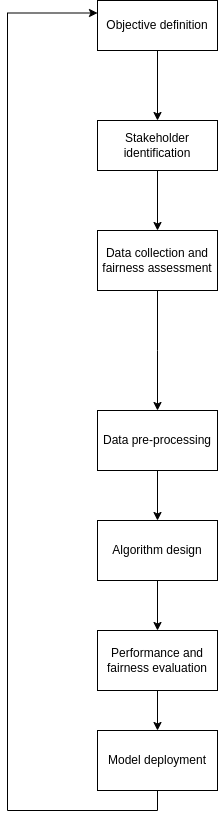
\includegraphics[width=.5\textwidth,height=1\textwidth]{final.png}
    \caption{Fair-by-Design Workflow}
\end{figure}

In the subsequent sections, each of these steps will be comprehensively explored to provide a detailed understanding of the fair-by-design workflow and its ethical underpinnings.

\section{Objective Definition}
\label{section:objective-definition}

The inaugural stage of a fair-by-design workflow mandates the meticulous definition of the system's objectives. The clarity and precision with which these objectives are articulated play a pivotal role in shaping subsequent design decisions. Within the realm of fairness, it becomes imperative to explicitly integrate fairness considerations into the articulated objectives.

In setting the system's goals, a nuanced understanding of the broader ethical landscape becomes foundational. This includes a comprehensive grasp of the potential societal impact, the diverse user base, and the nuanced interplay of ethical considerations within the specific domain of application. The deliberate inclusion of fairness considerations at this early juncture ensures that the pursuit of system objectives aligns seamlessly with the overarching ethical principles, reflecting a commitment to equitable and unbiased outcomes.

By explicitly weaving fairness into the fabric of the defined objectives, the fair-by-design approach underscores its commitment to the proactive anticipation and mitigation of biases. This foundational step lays the groundwork for subsequent design choices, framing the entire development process within an ethical framework that prioritizes fairness and aligns with societal values.

\subsection{Key Considerations}

\begin{enumerate}

    \item \emph{Clarity and Precision:}

        \begin{itemize}

            
            \item \emph{Precision in Objective Definition:} The formulation of specific objectives for the system or process demands clarity and precision to establish a focused and effective approach. This entails articulating goals that are both clear and measurable, aligning seamlessly with the overarching purpose of the system. Objectives should strive to eliminate ambiguity, providing a concrete understanding of the system's intended achievements. 
            
            The significance of clarity in objectives extends beyond the initial definition phase. It serves as a guiding beacon throughout the subsequent development and implementation processes, ensuring a cohesive and purposeful trajectory. Furthermore, the articulation of unambiguous objectives facilitates the accurate evaluation of the system's success in attaining its intended goals. This commitment to precision in objective definition not only enhances the effectiveness of the system but also contributes to a more robust and evaluative framework for assessing its overall impact and success.
            
            \item \emph{Comprehensive Articulation of System Attributes:} A foundational aspect of the fair-by-design workflow involves the explicit and detailed articulation of the system's intended functionalities, goals, and expected outcomes. This comprehensive elucidation is indispensable for fostering a profound understanding of the system or process.

            The delineation of functionalities necessitates a detailed description, outlining the specific tasks or operations the system is designed to execute. Precision in stating goals becomes paramount, emphasizing the overarching aims that the system aspires to achieve. Additionally, the expected outcomes must be clearly defined, specifying the anticipated results or benefits that stakeholders can expect from the successful implementation of the system.
            
            This level of clarity ensures a seamless alignment between development efforts and the envisioned impact, facilitating effective communication and collaboration among all involved parties. By providing a robust framework of understanding, this articulation of functionalities, goals, and outcomes becomes instrumental in guiding subsequent design decisions and ensuring that the fair-by-design approach remains steadfast in its commitment to transparent and equitable system development.        
        
        \end{itemize}
    
    \item \emph{Incorporating Fairness:}

        \begin{itemize}
            
            \item \emph{Explicit Emphasis on Fairness:} A paramount facet in the fair-by-design workflow involves the explicit and emphatic statement of the importance of fairness in achieving the defined objectives. Fairness is not merely an auxiliary consideration; it stands as a foundational principle that underpins the ethical and equitable functioning of the system.

            By explicitly prioritizing fair treatment for all individuals or groups affected by the system, it serves as a cornerstone for enhancing trust, mitigating potential biases, and promoting inclusivity. This acknowledgment of fairness as a non-negotiable element in the pursuit of objectives reflects a resolute commitment to ethical practices and responsible deployment.
            
            Furthermore, positioning fairness as a critical consideration aligns the system with societal values, legal standards, and stakeholder expectations. This alignment not only fosters a positive impact on the system's performance but extends to its broader social implications. The explicit emphasis on fairness within the fair-by-design framework signifies a dedication to cultivating technology that not only meets its functional objectives but does so with a keen awareness of the ethical imperatives that define its relationship with the individuals and communities it serves.
                                    
            \item \emph{Alignment of Fairness with System Purpose:} The seamless alignment of fairness with the overarching purpose of the system is an integral determinant of its effectiveness and societal impact. Fairness ensures that the system operates in a manner characterized by justice, impartiality, and a consideration of diverse perspectives. In this alignment, fairness becomes a cornerstone for enhancing the legitimacy of outcomes, promoting equal opportunities, and guarding against discriminatory practices.

            Incorporating fairness as a core element within the system not only facilitates the ethical attainment of defined objectives but also contributes significantly to cultivating a more inclusive and equitable societal framework. Fairness becomes a driving force that not only strengthens the system's purpose but also fosters trust and positive engagement among users and stakeholders. Simultaneously, it serves as a proactive safeguard, minimizing negative consequences and disparities that may arise from the system's operations.
            
            In essence, the intentional integration of fairness aligns the system with a broader ethical compass, elevating its purpose beyond mere functionality to a realm where societal impact is inherently intertwined with principles of justice, equity, and ethical responsibility.

        \end{itemize}
    
    \item \emph{Balancing Objectives:}

        \begin{itemize}
            
            \item \emph{Balancing Multiple Objectives with Fairness:} Striking a delicate balance among various objectives is paramount, demanding meticulous consideration to prevent the compromise of fairness in the pursuit of other goals. While the system may encompass multifaceted objectives such as efficiency, accuracy, and speed, the commitment to fairness should remain unwavering.

            This delicate equilibrium requires optimizing the system to meet its diverse goals without perpetuating biases or causing harm to specific groups. It necessitates a nuanced approach, where trade-offs are carefully evaluated to ensure that fairness is not sacrificed for the sake of expediency or efficiency. By upholding fairness as a foundational principle, the system can achieve a harmonious equilibrium, fostering an environment where diverse objectives are met without undermining the ethical considerations embedded in the pursuit of those objectives.

            This commitment to balance not only enhances the ethical standing of the system but also contributes to the creation of a technology landscape where fairness is not an afterthought but an integral and non-negotiable aspect of system optimization. In navigating these complexities, the fair-by-design framework becomes a guiding compass, ensuring that the pursuit of efficiency and other objectives remains harmonized with the overarching commitment to fairness.
            
            \item \emph{Identifying Conflicts and Establishing Priorities:} In navigating the intricate landscape of system development, a crucial undertaking involves identifying potential conflicts and establishing priorities among competing objectives. While fairness stands as a paramount consideration, it may at times seem to conflict with other objectives such as efficiency or cost-effectiveness. In such scenarios, conducting a thorough analysis becomes imperative to discern the nature and extent of these conflicts.

            Establishing clear priorities involves a meticulous assessment of the relative importance of each objective and determining where compromises can be made without jeopardizing the ethical principles underpinning fairness. This process demands a careful weighing of trade-offs, with the ultimate goal of aligning competing objectives in a manner that upholds fairness as a non-negotiable priority while still achieving overall system efficiency and effectiveness.
            
            The pursuit of these priorities is not a one-size-fits-all endeavor but requires a nuanced understanding of the specific context and ethical implications. By engaging in this deliberate process of conflict resolution and priority establishment, the fair-by-design workflow ensures that fairness remains at the forefront, serving as a guiding principle that shapes the overall development trajectory of the system.

        \end{itemize}

\end{enumerate}

\subsection{Detailed Implementation Steps}

\subsubsection{Stakeholder Engagement}

\begin{itemize}

    \item \emph{Objective Setting Through Stakeholder Engagement:} The definition of objectives within the fair-by-design workflow is a collaborative and inclusive process that begins by engaging key stakeholders, including end-users, developers, and decision-makers. This fundamental step fosters a collective and participatory approach to system development, where the diverse perspectives and insights of stakeholders are incorporated into the objective-setting process.

    End-users, with their real-world experience, provide valuable input rooted in practical needs. Developers contribute technical expertise, and decision-makers bring strategic considerations to the table. This collective engagement ensures not only a comprehensive understanding of the system's purpose but also enhances the likelihood of creating a solution that aligns with the varied requirements and expectations of all involved parties.

    The collaborative foundation established through stakeholder engagement is essential for achieving consensus on objectives. This consensus, in turn, paves the way for the successful development and implementation of a fair and effective system. By involving stakeholders from the outset, the fair-by-design workflow acknowledges the richness of diverse perspectives, fostering a sense of ownership and collective responsibility in the pursuit of objectives that are both ethically grounded and practically relevant.\item \emph{Objective Setting Through Stakeholder Engagement:} The definition of objectives within the fair-by-design workflow is a collaborative and inclusive process that begins by engaging key stakeholders, including end-users, developers, and decision-makers. This fundamental step fosters a collective and participatory approach to system development, where the diverse perspectives and insights of stakeholders are incorporated into the objective-setting process.

    End-users, with their real-world experience, provide valuable input rooted in practical needs. Developers contribute technical expertise, and decision-makers bring strategic considerations to the table. This collective engagement ensures not only a comprehensive understanding of the system's purpose but also enhances the likelihood of creating a solution that aligns with the varied requirements and expectations of all involved parties.

    The collaborative foundation established through stakeholder engagement is essential for achieving consensus on objectives. This consensus, in turn, paves the way for the successful development and implementation of a fair and effective system. By involving stakeholders from the outset, the fair-by-design workflow acknowledges the richness of diverse perspectives, fostering a sense of ownership and collective responsibility in the pursuit of objectives that are both ethically grounded and practically relevant.
    
    \item \emph{Implementation:}

        \begin{itemize}
            
            \item Conduct stakeholder interviews, surveys, or workshops to gather insights into their expectations and requirements.
            
            \item Ensure diverse representation to capture a comprehensive range of perspectives.
            
            \item Facilitate open discussions to uncover implicit biases or preferences that may influence objectives.
        
        \end{itemize}

\end{itemize}

\subsubsection{Define Performance Metrics}

\begin{itemize}

    \item \emph{Objective:} Specify the metrics that will serve as the yardstick for measuring the success of the system, ensuring a well-defined and quantitative framework for evaluation. These metrics should be meticulously selected to align with the established objectives, encompassing both technical performance and fairness considerations.

    For technical aspects, metrics such as accuracy, precision, recall, and F1 score may be relevant, providing insights into the system's overall effectiveness. Simultaneously, metrics specifically designed to assess fairness, such as disparate impact, equalized odds, and overall fairness indices, should be included to gauge the system's fairness.
    
    The chosen metrics must accurately reflect the intended outcomes and contribute to a comprehensive assessment, enabling a nuanced understanding of the system's success. Upholding fairness as a paramount criterion, the fair-by-design approach ensures that the selected metrics go beyond traditional performance indicators, providing a holistic evaluation that considers both technical proficiency and ethical considerations. This commitment to a diverse set of metrics facilitates a comprehensive understanding of the system's impact, fostering an environment where success is measured not only by technical prowess but also by the ethical principles embedded in the fair-by-design framework.    
    
    \item \emph{Implementation:}
        
    \begin{itemize}
            
        \item Identify traditional performance metrics (e.g., accuracy, precision, recall) relevant to the system's goals.
            
        \item Integrate fairness-specific metrics, such as disparate impact, equalized odds, or statistical parity, depending on the context.
            
        \item Establish a comprehensive set of metrics that collectively address both general system performance and fairness considerations.

    \end{itemize}

\end{itemize}

\subsubsection{Ethical Considerations}

\begin{itemize}

    \item \emph{Objective:} Undertake a comprehensive exploration of the ethical implications associated with the defined objectives, conducting a thorough examination to anticipate and address potential ethical challenges. This involves a deep dive into how the system's goals and functionalities may intersect with broader ethical considerations, including privacy, security, and societal impact.

    Consider the implications for different stakeholder groups, ensuring that the system's objectives align with ethical standards and societal values. This involves a proactive approach, articulating clear guidelines and safeguards to mitigate ethical concerns, thereby promoting transparency and accountability throughout the development and implementation phases.
    
    By proactively addressing ethical implications, the system positions itself to navigate complex ethical landscapes responsibly. This commitment to ethical foresight not only upholds ethical considerations alongside technical functionalities but also contributes to the creation of a technology-driven environment that prioritizes ethical principles. Through this conscientious approach, the fair-by-design workflow not only aims for technical excellence but also seeks to embed a strong ethical foundation, fostering a system that is not only proficient but also ethically responsible.

    \item \emph{Implementation:}

        \begin{itemize}

            \item Conduct an ethical impact assessment to identify potential biases or unintended consequences.

            \item Evaluate the ethical implications of each performance metric, ensuring alignment with fairness goals.

            \item Anticipate scenarios where ethical dilemmas may arise and establish guidelines for resolution.

        \end{itemize}

\end{itemize}

\subsubsection{Documentation}

\begin{itemize}

    \item \emph{Objective:} Rigorously document the defined objectives in a clear and comprehensive manner, ensuring that each objective is articulated with precision and detail. Provide a detailed overview of the intended functionalities, goals, and expected outcomes, leaving no room for ambiguity.

    Utilize concise and unambiguous language to capture the essence of each objective, outlining the specific tasks or functionalities the system aims to achieve. Include any relevant context or background information that enhances the understanding of each objective. This documentation serves as a foundational reference for all stakeholders involved in the development and implementation of the system.

    The goal is to foster a shared understanding of the project's overarching goals and guiding principles among team members, end-users, and decision-makers throughout the system's lifecycle. Clarity and comprehensiveness in objective documentation are indispensable for effective communication and collaboration. By meticulously documenting the objectives, the fair-by-design workflow not only ensures alignment with ethical principles but also establishes a robust foundation for informed decision-making and collective engagement across all stages of system development.
    
    \item \emph{Implementation:}

        \begin{itemize}

            \item Create a detailed objective statement that serves as a reference point for all stakeholders.

            \item Document the rationale behind the inclusion of fairness considerations in the objectives.

            \item Maintain a living document that can be updated as objectives evolve or new insights emerge.

        \end{itemize}

\end{itemize}

\subsection{Significance}

Defining objectives with precision, incorporating fairness considerations, and establishing clear performance metrics are the foundational pillars of a fair-by-design approach. Precision in objective definition is crucial to avoid ambiguity and guide the development process effectively. Integrating fairness considerations from the outset ensures that ethical principles are not an afterthought but integral to the system's purpose. Clear performance metrics enable the systematic evaluation of the system's success and adherence to fairness goals.

Together, these steps create a comprehensive framework that not only aligns the system with ethical standards but also meets stakeholder expectations, fostering trust and accountability throughout the development lifecycle. This approach not only enhances the effectiveness of the system but also contributes to a technology landscape where ethical considerations are seamlessly woven into the fabric of technological advancements. Through a meticulous and proactive fair-by-design methodology, the system becomes not just a product of technical prowess but a testament to ethical responsibility and societal relevance.

\section{Stakeholder Identification}
\label{section:stakeholder-identification}

Engaging key stakeholders is a foundational step in shaping the objectives of a fair-by-design workflow. Stakeholders, representing diverse perspectives and interests, bring invaluable insights that contribute to defining the system's purpose. Involving a range of stakeholders ensures a comprehensive understanding of ethical implications and societal expectations. This inclusive approach not only fosters a sense of collective responsibility but also helps in addressing potential biases and concerns early in the design process.

By incorporating various viewpoints, the fair-by-design workflow becomes more attuned to the needs of different communities and stakeholders, enhancing the overall fairness and effectiveness of the system. This collaborative engagement not only contributes to the ethical grounding of the system but also establishes a sense of shared ownership and accountability among stakeholders. Through this inclusive approach, the fair-by-design methodology ensures that the development process is enriched by a diversity of perspectives, making the resulting system more responsive, transparent, and aligned with the values and expectations of the broader community it serves.

\subsection{Key Considerations}

\begin{enumerate}

    \item \emph{Diverse Representation:}

        \begin{itemize}

            \item \emph{Ensuring Inclusive Stakeholder Representation:} In the fair-by-design approach, ensuring the inclusion of stakeholders who represent a diverse range of perspectives is paramount. This encompasses stakeholders such as end-users, developers, decision-makers, and members of affected communities. Each stakeholder group contributes unique insights and experiences that are crucial for shaping a system that is equitable and aligned with ethical principles.

            End-users provide practical insights into how the system will be experienced, developers offer technical expertise, decision-makers provide strategic guidance, and affected communities bring perspectives on potential societal impacts. By actively involving this diverse set of stakeholders, the fair-by-design workflow gains a more holistic understanding of potential biases, ethical considerations, and the broader societal context, ultimately leading to a more inclusive and equitable outcome.
            
            This intentional inclusion of diverse voices not only enhances the fairness of the system but also establishes a collaborative foundation that reflects a commitment to responsible and ethical AI development. The fair-by-design methodology recognizes the significance of varied perspectives in creating technology that not only functions effectively but also considers the diverse needs and impacts on the communities it serves.

        \end{itemize}
    
    \item \emph{Inclusive Decision-Making:}
        
    \begin{itemize}
    
        \item \emph{Fostering Inclusive Decision-Making:} Fostering an inclusive environment is integral to the fair-by-design approach, ensuring that stakeholders actively participate in decision-making processes related to the system's objectives. This inclusivity encourages diverse perspectives, fostering a collaborative atmosphere where each stakeholder's input is valued.

        Establishing open channels of communication and providing opportunities for meaningful engagement empowers stakeholders to contribute their insights effectively. By creating an inclusive space, the fair-by-design workflow not only captures a broader range of perspectives but also cultivates a sense of ownership among stakeholders. This collaborative decision-making process enhances transparency, builds trust, and ultimately results in a system that is more responsive to the needs and values of the varied stakeholders involved.
        
        Through active and inclusive participation, stakeholders become co-creators of the system, contributing to its development in a manner that reflects a shared commitment to fairness and ethical considerations. This inclusive decision-making not only strengthens the ethical foundation of the system but also fosters a collaborative culture that extends beyond the development phase, influencing the ongoing relationship between the technology and the diverse communities it serves.

    \end{itemize}
    
    \item \emph{Transparent Communication:}
    
    \begin{itemize}

        \item \emph{Maintaining Transparent Communication Channels:} In the fair-by-design approach, maintaining transparent communication channels is crucial to keeping stakeholders informed about the development process and gathering their input effectively. Transparent communication fosters trust and ensures that stakeholders are aware of the system's progress, objectives, and any potential implications.

        Regular updates, clear documentation, and accessible information contribute to an open dialogue, allowing stakeholders to stay engaged and provide valuable feedback. This proactive approach to communication not only enhances the collaborative decision-making process but also promotes a shared understanding of the ethical considerations embedded in the system.
        
        Transparent communication channels serve as a cornerstone of the fair-by-design workflow, fostering a sense of inclusivity and shared responsibility among all stakeholders involved. By keeping the lines of communication open, the fair-by-design methodology not only embraces diverse perspectives but also actively engages stakeholders in a continuous dialogue that extends throughout the system's lifecycle. This commitment to transparency is instrumental in building and sustaining trust, creating an environment where stakeholders feel empowered and informed in their roles as contributors to the ethical development of the technology.

    \end{itemize}

\end{enumerate}

\subsection{Detailed Implementation Steps}

\subsubsection{Stakeholder Mapping}

\begin{itemize}
    
    \item \emph{Objective:} Identifying and mapping key stakeholders is a crucial step in the fair-by-design approach to understand and incorporate diverse perspectives in the system's development. Key stakeholders include end-users, developers, decision-makers, and affected communities, each bringing unique insights and interests to the table.

    End-users provide valuable feedback based on their experiences and expectations, guiding user-centric design. Developers contribute technical expertise, ensuring the feasibility and efficiency of the system. Decision-makers offer strategic input aligning the system with broader organizational goals. Affected communities bring a contextual understanding of societal impacts, helping navigate ethical considerations.
    
    By mapping these stakeholders, the fair-by-design workflow ensures a holistic and inclusive approach, considering the varied interests and perspectives that shape the system's objectives and ethical considerations. This intentional identification and mapping process set the foundation for a collaborative and well-informed decision-making process, where the diverse voices of stakeholders are actively incorporated into the development trajectory of the system.

    \item \emph{Implementation:}
    
    \begin{itemize}
    
        \item Create a stakeholder map that identifies different stakeholder groups and their respective roles and interests.
    
        \item Prioritize stakeholders based on their influence on or impact from the system.
    
    \end{itemize}

\end{itemize}

\subsubsection{Engagement Strategies}

\begin{itemize}

    \item \emph{Objective:} Developing effective strategies for stakeholder engagement in the objective-setting process is pivotal for a fair-by-design workflow. Begin by conducting stakeholder analysis to identify key individuals and groups. Establish clear communication channels to disseminate information and gather feedback. Organize workshops, focus groups, or collaborative sessions to facilitate active participation. Tailor engagement methods to suit diverse stakeholders, ensuring inclusivity.

    Provide accessible documentation outlining the proposed objectives and ethical considerations. Emphasize the value of each stakeholder's input and foster an open dialogue to address concerns. Regularly update stakeholders on the progress, incorporating their feedback iteratively.
    
    By employing these strategies, a fair-by-design workflow ensures comprehensive engagement, enriching the objective-setting process with diverse perspectives and reinforcing ethical considerations. This proactive and inclusive approach to stakeholder engagement not only enhances the quality of the objectives but also contributes to a collaborative and transparent development process, where stakeholders feel valued and actively contribute to the ethical foundation of the system.

    \item \emph{Implementation:}

    \begin{itemize}

        \item Tailor engagement strategies to the characteristics of each stakeholder group (e.g., workshops, surveys, focus groups).

        \item Clearly communicate the importance of their input in shaping the ethical foundations of the system.

    \end{itemize}

\end{itemize}

\subsubsection{Inclusive Workshops or Meetings}

\begin{itemize}

    \item \emph{Objective:} In fostering an inclusive fair-by-design approach, organizing workshops or meetings is instrumental for stakeholder engagement in defining objectives. These sessions provide a platform for active participation, allowing diverse stakeholders, including end-users, developers, decision-makers, and affected communities, to contribute insights.

    The workshops should be designed to encourage open dialogue, ensuring that each perspective is heard and considered. Employ facilitation techniques that promote inclusivity, such as structured discussions, brainstorming sessions, or collaborative activities. By facilitating these inclusive workshops, the fair-by-design workflow embraces diverse viewpoints, enriching the objective-setting process and reinforcing its commitment to ethical considerations.
    
    Through these workshops, the fair-by-design methodology actively encourages a collaborative environment where stakeholders feel empowered to contribute, fostering a sense of ownership and shared responsibility in shaping the system's objectives. This inclusive approach not only enhances the quality of the objectives but also establishes a foundation for continued collaboration and engagement throughout the development lifecycle.

    \item \emph{Implementation:}

    \begin{itemize}

        \item Organize collaborative sessions that encourage open dialogue and the exchange of diverse perspectives.

        \item Provide a platform for stakeholders to express their values, concerns, and expectations related to fairness in the system.

    \end{itemize}

\end{itemize}

\subsubsection{Feedback Collection}

\begin{itemize}

    \item \emph{Objective:} After defining initial objectives and ethical considerations in the fair-by-design workflow, it is crucial to gather feedback from stakeholders. Establish a feedback loop through surveys, interviews, or focus group discussions to ensure that the proposed objectives resonate with the diverse perspectives of stakeholders. This iterative process allows for refinements and adjustments based on the input received.

    Actively seeking feedback fosters collaboration and ensures that the fair-by-design approach remains responsive to the evolving needs and expectations of stakeholders throughout the system's development. This ongoing feedback loop not only contributes to the iterative improvement of objectives but also reinforces a culture of continuous engagement, where stakeholders play an active role in shaping the ethical foundation of the technology.

    \item \emph{Implementation:}

    \begin{itemize}

        \item Utilize surveys, interviews, or online platforms to collect structured feedback.

        \item Encourage stakeholders to provide qualitative insights that may not be captured by quantitative methods.

    \end{itemize}

\end{itemize}

\subsection{Significance}

Stakeholder identification is a pivotal aspect of ensuring the fair and inclusive development of a system. Involving stakeholders from diverse backgrounds and perspectives allows the ethical considerations embedded in the objectives to more accurately reflect the values and expectations of the broader community. By recognizing and engaging with a variety of stakeholders, including end-users, developers, decision-makers, and representatives from affected communities, the fair-by-design approach becomes more comprehensive and responsive to the multifaceted needs and concerns of the people who will interact with or be impacted by the system.

This inclusive process contributes to the development of a system that is not only technically sound but also ethically grounded and considerate of various societal perspectives. The intentional involvement of diverse stakeholders ensures that the resulting technology aligns with ethical standards and is more likely to meet the expectations of the communities it serves, fostering a sense of trust and accountability in the development process.

\section{Data Collection: Integration with Stakeholder Considerations}
\label{section:data-collection}

In the process of data collection, the integration of insights from stakeholders is crucial, particularly for the identification of protected attributes. Stakeholders bring valuable perspectives on societal norms, ethical considerations, and potential biases that may not be apparent solely from the dataset. Their input aids in defining and recognizing protected attributes, contributing to a more nuanced understanding of fairness in the context of the application.

Stakeholder involvement ensures that the identification of protected attributes is not solely based on technical or algorithmic considerations but is informed by the broader societal context. This inclusive approach helps uncover potential biases and ethical implications that might be overlooked in the data, leading to a more robust and ethically grounded system. By actively incorporating stakeholder insights in the identification of protected attributes, the fair-by-design methodology enhances the fairness and accountability of the system, aligning it more closely with the values and expectations of the diverse communities it serves.

\subsection{Importance of Stakeholder Integration}

\subsubsection{Cultural Sensitivity}

Stakeholders, representing diverse backgrounds, contribute significantly to a nuanced understanding of cultural norms and sensitivities within the fair-by-design approach. This diversity is crucial in recognizing attributes that may be culturally significant and warrant protection. For instance, certain cultural or religious practices may involve sensitive information that should be identified as a protected attribute to ensure respectful and unbiased treatment.

By actively involving stakeholders who bring a range of cultural perspectives, the objective-setting process can identify and address potential biases associated with cultural attributes, fostering a system that respects and reflects the rich diversity of its user base. This approach not only enhances fairness but also promotes cultural sensitivity and inclusivity in the design and implementation of the system.

Through the fair-by-design methodology, cultural considerations become integral to the ethical framework, ensuring that the system acknowledges and respects the cultural context of its users. This not only aligns the technology with ethical standards but also contributes to a more inclusive and culturally aware development process, ultimately leading to a system that is more equitable and considerate of the diverse cultural backgrounds of its users.

\subsubsection{Contextual Relevance}

Stakeholders play a crucial role in providing contextual insights that may not be evident in the dataset alone within the fair-by-design approach. Their considerations can guide the identification of attributes relevant to the specific application and its ethical implications. For instance, in an educational context, stakeholders might highlight attributes related to socio-economic status or learning styles that could impact fairness considerations in student evaluations.

By actively involving stakeholders, the objective-setting process gains valuable perspectives that enrich the ethical framework of the system. This collaborative approach ensures that the identified objectives not only align with technical requirements but also address real-world considerations, promoting a more holistic and socially responsible system.

Through the fair-by-design methodology, stakeholders become partners in shaping a system that is not only technically robust but also considerate of the diverse and dynamic factors influencing its ethical considerations. This inclusive collaboration helps bridge the gap between technical requirements and real-world implications, fostering a technology landscape that is not only advanced but also socially conscious and responsive to the needs and concerns of the communities it serves.

\subsubsection{Uncovering Implicit Biases}


Stakeholders play a crucial role in uncovering implicit biases that may not be explicitly represented in the dataset within the fair-by-design approach. By incorporating their perspectives, the identification of protected attributes becomes more comprehensive and reflective of potential sources of bias. This is particularly important in domains where historical biases or societal prejudices might influence decision-making processes.

Stakeholders can provide valuable input to address and mitigate these implicit biases, contributing to the development of a more equitable and unbiased system. Their involvement ensures a thorough examination of potential biases, fostering transparency and fairness in the system's design and objectives.

Through the fair-by-design methodology, stakeholders act as critical agents in the identification and mitigation of biases, leading to a more robust and ethically grounded system. This collaborative approach not only enhances the fairness of the technology but also promotes a culture of accountability and transparency in addressing biases that may exist in the underlying data or decision-making processes.

\subsection{Implementation Steps}

\subsubsection{Stakeholder Workshops}

\emph{Objective:} Integrate stakeholder considerations into the identification of protected attributes.

\emph{Implementation:}

\begin{itemize}

    \item Conduct stakeholder workshops specifically focused on discussing and identifying potential protected attributes.

    \item Encourage open discussions to uncover implicit biases or attributes that may have societal implications.

    \item Facilitate collaboration between data scientists and stakeholders to ensure a shared understanding of fairness goals.

\end{itemize}

\subsubsection{Documentation of Stakeholder Input}

\emph{Objective:} Document stakeholder input on protected attributes for transparency.

\emph{Implementation:}

\begin{itemize}

    \item Record the insights shared by stakeholders regarding attributes they perceive as sensitive or requiring protection.

    \item Incorporate stakeholder considerations into the broader documentation of the data collection process.

    \item Provide clear documentation of the integration process to maintain transparency and facilitate reproducibility.

\end{itemize}

\section{Data Pre-processing}
\label{section:pre-proc}

Following the completion of data collection and the incorporation of stakeholder considerations, the subsequent pivotal stage in the workflow is data pre-processing. This critical phase is dedicated to meticulously preparing and cleansing the dataset with the overarching goal of addressing biases, rectifying imbalances, and ensuring a fair and equitable foundation for the ensuing stages of the fair-by-design workflow. The emphasis during data pre-processing is on refining the dataset to foster a more equitable and unbiased representation, thus laying the groundwork for robust and ethical data-driven decision-making processes.

\subsection{Key Considerations}

\begin{enumerate}

    \item \emph{Data cleaning:} 

    This process involves identifying and rectifying errors, inconsistencies, and inaccuracies in the raw dataset to ensure its reliability and quality. Common tasks in data cleaning include handling missing values, correcting data format issues, removing duplicates, and addressing outliers. The goal is to create a clean, standardized dataset that forms a solid foundation for subsequent analysis and model development. Rigorous data cleaning is essential for mitigating the risk of biased or inaccurate model outcomes, as machine learning models heavily depend on the quality of the input data. This meticulous attention to data quality sets the stage for effective feature engineering, model training, and, ultimately, the generation of reliable and fair predictions.

    \item \emph{Handling Protected Attributes:} 
    
    Within the Fair-by-Design workflow, categorical protected attributes undergo a transformation process to ensure fairness in subsequent machine learning stages. This process involves setting a threshold for each protected attribute and replacing values above the threshold with 1, and values below the threshold with 0.

    Let \(P\) be the set of protected attributes, and \(p_i\) represent a specific protected attribute within \(P\). The threshold, denoted as \(t_i\), is determined for each categorical protected attribute \(p_i\) in the dataset through the following formalism:

    \[
    t_i = \frac{\text{min}(p_i) + \text{max}(p_i)}{2}
    \]

    This calculation ensures a nuanced understanding of the prevalent categories within these attributes and establishes a threshold \(t_i\) for distinguishing between them.

    The binary representation preserves essential information about protected attributes, providing a condensed yet informative encoding that reflects the privilege or lack thereof concerning specific attributes.

    During the training phase, the model learns to distinguish instances based on privilege or lack thereof concerning specific attributes, as represented by the binary encoding. This is achieved by replacing values according to the following transformation:

    \[
    \text{Binary Encoding}(p_i) = \begin{cases} 

        1 & \text{if } p_i > t_i \\

        0 & \text{if } p_i \leq t_i 

    \end{cases}
    \]

    This facilitates effective model incorporation and decision-making during training and prediction phases.

    The nuanced encoding strategy, where values over the threshold are replaced with 1 and values under the threshold are replaced with 0, serves as the foundation for unbiased and fair treatment of instances within the model. By transforming categorical protected attributes based on the specified threshold definition, the Fair-by-Design workflow ensures that subsequent machine learning models can effectively incorporate and act upon this information during training and prediction phases, contributing significantly to the development of a more equitable and ethically sound machine learning model.

    \item \emph{Handling Output Variable:} 
    
    The handling of the output variable in the Fair-by-Design workflow is a nuanced process that adapts to the nature of the variable, whether categorical or continuous. This tailored treatment is essential for aligning the prediction task with the fairness objectives of the workflow, ensuring that the model's predictions are not only accurate but also ethically sound.


    In cases where the output variable is categorical, the workflow initiates by determining the most frequent value within this category. Let $Y$ represent the output variable, and $y_i$ be a specific outcome within $Y$. The most frequent value, denoted as $y_{\text{freq}}$, is determined through the following formalism:

    \[
    y_{\text{freq}} = \text{argmax}_y \left( \text{count}(Y = y) \right)
    \]

    This strategic calculation provides insights into the prevailing outcome within the dataset. Subsequently, instances where the output variable matches $y_{\text{freq}}$ are replaced with the binary representation 1, while all other instances take on the binary representation 0. The binary encoding function is defined as follows:

    \[
    \text{Binary Encoding}(y_i) = \begin{cases} 
    1 & \text{if } y_i = y_{\text{freq}} \\ 
    0 & \text{otherwise}
    \end{cases}
    \]

    This transformation effectively redefines the prediction task, shifting the focus to discerning whether a given sample belongs to the most frequent outcome. The binary encoding approach not only simplifies the representation of categorical outcomes but also enables the model to make predictions in a manner that aligns with fairness considerations.


    Conversely, when the output variable is continuous, the workflow employs a distinct strategy. Let $Z$ represent the continuous output variable, and $z_i$ be a specific value within $Z$. Values of the continuous variable that surpass the mean are replaced with 1, while those falling below the mean assume the binary representation 0. This adjustment transforms the prediction task into establishing whether a sample's continuous output is above the mean. The binary encoding function for continuous variables is defined as:

    \[
    \text{Binary Encoding}(z_i) = \begin{cases} 
    1 & \text{if } z_i > \text{mean}(Z) \\ 
    0 & \text{otherwise}
    \end{cases}
    \]

    This approach ensures that the model is not only attentive to the central tendency of the continuous variable but also considers the distribution of values concerning the mean.

    This tailored and meticulous treatment of the output variable underscores the commitment of the Fair-by-Design workflow to equitable and ethical machine learning practices. The workflow not only adapts to the inherent characteristics of the data but also ensures that the subsequent model operates with a heightened awareness of fairness considerations, contributing to the development of a more responsible and unbiased machine learning model.

\end{enumerate}

This nuanced pre-processing step sets the groundwork for a fair and unbiased learning prediction, aligning the dataset with the ethical considerations embedded in the Fair-by-Design workflow.

\section{Algorithm Design}
\label{section: algorithm-design}

The stage of Algorithm Design within the fair-by-design workflow stands as a pivotal phase wherein the selection, adaptation, or creation of machine learning models takes place to harmonize with the specified objectives and fairness considerations. The primary objective is to craft models that not only excel in accuracy but also steadfastly adhere to ethical and fair principles. This section undertakes an in-depth exploration of the crucial considerations, strategic approaches, and the step-by-step implementation processes entailed in Algorithm Design. By navigating through these aspects, the aim is to foster the development of models that not only deliver superior performance but also champion the ideals of ethics and fairness in their predictive outcomes.

\subsection{Key Considerations}

\begin{enumerate}

    \item \emph{Fairness-Aware Model Selection:} 
    
    The selection of machine learning models assumes a pivotal role in the pursuit of fairness objectives. Fairness-aware model selection entails the deliberate consideration of models equipped with inherent mechanisms to tackle biases and advocate for equitable outcomes. Noteworthy examples of such models include adversarial networks, fairness-aware classifiers, and re-weighted learning algorithms. These models are systematically explored and evaluated for their capacity to mitigate biases and foster fairness, thereby contributing to the overarching goal of cultivating just and impartial predictive systems.
    
    \item \emph{Regularization Techniques:} 
    
    In the pursuit of fair predictions, regularization methods, exemplified by demographic parity constraints or equalized odds constraints, emerge as instrumental tools. These methodologies are strategically employed to guide machine learning models towards fairness objectives. By integrating fairness constraints into the optimization process, these regularization techniques play a pivotal role in steering the model to yield equitable outcomes across various demographic groups. The inclusion of such constraints serves as a proactive measure to counteract biases and ensure that the predictive power of the model remains impartial and just across diverse demographic contexts.

    \item \emph{Bias Detection and Mitigation:} 
    
    The integration of embedding mechanisms within the algorithm to detect and mitigate biases is of paramount importance. This entails the ongoing and systematic monitoring of the model's predictions for any indications of disparate impact. Subsequently, corrective measures are implemented in real-time to mitigate biases as they manifest. This proactive approach to bias detection and mitigation serves as a fundamental component in ensuring the model's fairness and equity. By embedding mechanisms that facilitate continuous scrutiny and timely interventions, the algorithm is fortified to deliver more impartial and just predictions, aligning with the principles of ethical and fair machine learning.

    \item \emph{Pre-processing, In-processing, or Post-processing Algorithms:} 
    
    The strategic decision regarding the selection of pre-processing, in-processing, or post-processing algorithms is intricately tied to the specific characteristics of the data and the defined fairness goals. Pre-processing algorithms, characterized by their ability to transform the dataset prior to model training, set the initial conditions for fairness considerations. In-processing algorithms, on the other hand, directly modify the learning process during model training, introducing fairness mechanisms at this crucial stage. Post-processing algorithms, as the name implies, come into play after model training, adjusting predictions to align with fairness objectives.

    When making this strategic decision, it is imperative to consider the nature of biases inherent in the data, the characteristics of the available dataset, and the desired level of fairness. Each approach—pre-processing, in-processing, or post-processing—offers distinct advantages and considerations, and the choice among them should be informed by a comprehensive understanding of the specific fairness challenges and objectives inherent to the machine learning task at hand.

\end{enumerate}

\subsection{Detailed Implementation Steps}

% Include the detailed implementation steps for each key consideration as per the previous discussion.

\subsubsection{Fairness-Aware Model Selection}

\begin{itemize}

    \item \emph{Exploration of Fairness-Aware Models:}
     
    \begin{itemize}
    
        \item In the endeavor to develop a fair-by-design machine learning model, a pivotal step involves conducting an exhaustive survey and evaluation of existing fairness-aware models tailored to the specific application domain. This meticulous process requires a thorough examination of pertinent literature and available models, taking into account their performance metrics, interpretability, and fairness considerations. By subjecting existing models to rigorous evaluation, practitioners gain valuable insights into the nuanced strengths and limitations of different approaches. This discerning survey and evaluation process empower practitioners to make informed decisions regarding the most suitable model for their particular use case. Such diligence contributes significantly to the foundational aspects of a fair-by-design workflow, ensuring that the selected model not only aligns with technical requirements but also upholds ethical considerations inherent to the application domain.
    
        \item When delving into the realm of fairness-aware models tailored for a specific application domain, it is judicious to prioritize models explicitly designed to address bias. This consideration encompasses, but is not confined to, adversarial networks or models featuring inherent fairness constraints. Adversarial networks serve the purpose of mitigating bias by introducing a secondary network that identifies and counteracts any discriminatory patterns discerned in the primary model. Conversely, models with built-in fairness constraints integrate predefined fairness metrics into the optimization process, ensuring the model adheres to fairness criteria throughout training.

        The evaluation of these specialized models yields a nuanced understanding of their efficacy in handling bias, furnishing practitioners with invaluable insights into the most suitable approach for mitigating bias within their specific context. This deliberate consideration solidifies the fair-by-design approach, underscoring the paramount importance of selecting models that actively address and rectify biases to foster equitable outcomes in the realm of machine learning applications.    
    
    \end{itemize}
    
    \item \emph{Implementation and Customization:}
    
    \begin{itemize}
    
        \item Following the selection of a fairness-aware model tailored for the specific application domain, the subsequent imperative involves its implementation within the chosen machine learning framework. This intricate process necessitates the translation of model specifications and architecture into code, meticulous configuration of essential parameters, and seamless integration into the overarching machine learning pipeline. The implementation procedure should strictly adhere to industry best practices and guidelines stipulated by the chosen framework, ensuring not only optimal performance but also seamless compatibility.

        Furthermore, developers must prioritize the interpretability of the model, recognizing that transparency is pivotal in comprehending how fairness considerations are intricately embedded within the system. The successful execution of the implementation phase represents a pivotal juncture in the fair-by-design workflow. It sets the groundwork for subsequent stages encompassing model training, rigorous evaluation, and eventual deployment, all underscored by an unwavering commitment to fostering equitable and unbiased machine learning outcomes.    
    
        \item Subsequent to the implementation of the chosen fairness-aware model, a pivotal phase entails customizing the model to harmonize with the unique characteristics of the dataset and the precise fairness objectives delineated earlier in the workflow. This customization process necessitates the fine-tuning of model parameters, adjustment of hyperparameters, and incorporation of features that aptly accommodate the nuanced intricacies present in the dataset.

        Moreover, developers may find it imperative to introduce specific fairness-oriented adjustments to the model's architecture. This ensures the model's adeptness in effectively handling and mitigating biases associated with protected attributes. Such meticulous and tailored customization stands as an indispensable step for optimizing the model's performance within the paradigm of the fair-by-design approach. Here, the overarching objective extends beyond technical excellence, encompassing the ethical imperative of delivering unbiased machine learning outcomes.    
    
    \end{itemize}

\end{itemize}

\subsubsection{Explainability and Interpretability}

\begin{itemize}

    \item \emph{Model Selection:}

    \begin{itemize}

        \item Within the fair-by-design workflow, the strategic choice of models renowned for their high explainability and interpretability holds paramount significance. Decision trees and rule-based models, celebrated for their inherent transparency, stand out as preferred choices in this context. The rationale underpinning this selection is deeply rooted in the commitment to transparency and accountability.

        Models characterized by easy interpretability empower stakeholders, including end-users and decision-makers, to comprehend the intricate decision-making processes. This transparency not only cultivates trust but also facilitates the identification and mitigation of any potential biases or fairness concerns embedded within the model. By deliberately opting for models with high explainability, the fair-by-design workflow aligns seamlessly with its overarching goal of cultivating machine learning systems that excel not only in technical robustness but also in ethical soundness, ensuring they are readily understandable by a diverse range of stakeholders.

        \item Within the fair-by-design workflow, when infusing fairness considerations into model selection, a critical aspect is to judiciously navigate the trade-offs between model complexity and interpretability. The optimal balance hinges significantly on the specific application requirements, playing a pivotal role in the decision-making process.

        Highly complex models, while potentially offering superior predictive performance, often come at the cost of diminished interpretability. Conversely, interpretable models such as decision trees or rule-based models may exhibit limitations in capturing intricate patterns present in the data. Striking the right balance becomes paramount; the fair-by-design approach is not solely concerned with ensuring fairness but also places a premium on transparency.
        
        Therefore, the strategic selection of models aligning with the interpretability needs of stakeholders while still meeting performance requirements becomes a key consideration in the design process. This deliberate and conscious decision-making process contributes significantly to the development of machine learning models that are not only fair but also understandable and accountable, embodying the principles of the fair-by-design approach.

    \end{itemize}

\end{itemize}

\subsubsection{Regularization Techniques}

\begin{itemize}

    \item \emph{Integration of Fairness Constraints:}

    \begin{itemize}

        \item The incorporation of fairness constraints mandates a nuanced comprehension of the precise fairness goals and metrics germane to the application domain. In the fair-by-design approach, there is a pronounced emphasis on the principled and systematic integration of these constraints into the machine learning model's training process. This deliberate embedding of fairness into the training regimen aims to mitigate biases and advocate for equitable outcomes.

        The overarching objective of the fair-by-design workflow extends beyond the mere delivery of accurate predictions. It is intricately woven with the commitment to ethical and fairness considerations, thereby contributing substantively to the cultivation of responsible and unbiased machine learning practices. This concerted effort reinforces the imperative of aligning machine learning models with ethical principles, ensuring they operate within a framework that prioritizes fairness and equity.

        \item Within the fair-by-design approach to machine learning, a pivotal facet involves the systematic experimentation with various regularization techniques. These methods, exemplified by demographic parity constraints or equalized odds constraints, assume a substantial role in the concerted effort to mitigate biases and champion fairness within machine learning models. Tailored to address specific fairness considerations linked to protected attributes, these techniques are meticulously designed to ascertain that the model's predictions remain uninfluenced by factors such as gender, race, or other sensitive attributes. This intentional and exploratory engagement with regularization techniques underscores the commitment to cultivating models that not only excel in predictive accuracy but also uphold the ethical imperative of fairness and equity.
    
    \end{itemize}

\end{itemize}

\subsubsection{Bias Detection and Mitigation}

\begin{itemize}
    
    \item \emph{Dynamic Bias Mitigation:}
    
    \begin{itemize}
    
        \item A proactive strategy within the fair-by-design framework involves the development of adaptive algorithms that dynamically adjust to emerging biases in the data. These algorithms are meticulously designed to engage in continuous monitoring and evaluation of the model's performance, adept at identifying any potential biases that may manifest during operational phases. The adaptive nature of these algorithms empowers them to dynamically tweak parameters or decision boundaries in response to emerging biases, thereby ensuring an ongoing commitment to fairness in real-world applications. This forward-thinking approach aligns seamlessly with the ethos of the fair-by-design framework, emphasizing not only initial fairness but also the continuous vigilance and adaptation necessary for sustained equity in machine learning outcomes.

        \item A pivotal step in the fair-by-design workflow involves the implementation of corrective measures, such as re-weighting or re-sampling, to actively mitigate biases as they are detected. As biases are identified through ongoing monitoring, these targeted corrective measures are strategically applied to address imbalances and promote fairness in the model's predictions. This iterative and adaptive approach not only acknowledges the inevitability of biases but also proactively works towards rectifying them, reinforcing the commitment to fairness and equity embedded within the fair-by-design methodology.

    \end{itemize}

\end{itemize}

\subsubsection{Human-in-the-Loop Approaches}

\begin{itemize}
    
    \item \emph{Stakeholder Collaboration:}
    
    \begin{itemize}
    
        \item Organize collaborative sessions with domain experts and stakeholders to delve into the intricacies of fairness considerations. These sessions serve as a platform for a comprehensive exploration of nuances related to fairness, leveraging the collective insights and expertise of domain specialists and key stakeholders. The aim is to foster a shared understanding of fairness challenges, identify contextual nuances, and coalesce diverse perspectives. Such collaborative endeavors contribute significantly to the fair-by-design approach, ensuring that the developed models align not only with technical requirements but also with the ethical and contextual considerations of the specific application domain.
    
        
        \item Engage stakeholders actively in both model validation and decision-making processes. This participatory approach ensures that the perspectives and insights of stakeholders are integral to the validation of the model's performance and the decision-making procedures. By involving stakeholders, including end-users and decision-makers, in these crucial stages, the fair-by-design workflow embraces transparency and inclusivity. This collaborative involvement contributes to the development of models that are not only technically sound but also align with the diverse needs and expectations of the stakeholders, fostering a sense of ownership and accountability in the overall machine learning process.
    
    \end{itemize}

\end{itemize}

\subsection{Pre-processing Algorithm Proposed}

\subsubsection{Fairness through data rebalancing}
\label{subsec:ftdr}

In this approach, the paradigm of bias mitigation takes on a unique and innovative perspective, one that prioritizes data augmentation over attribute removal. Unlike traditional approaches that center on the exclusion of specific attributes, this methodology embraces the concept of data augmentation, introducing a distinctive definition of fairness and equity within the AI system.

The essence of this approach revolves around the augmentation of the dataset by introducing new data instances that offer a more comprehensive and inclusive representation of the underlying population. This expanded dataset is designed to be more diverse, representative, and balanced, transcending the limitations of the original data and fostering a more nuanced understanding of fairness. 

The introduction of augmented data instances leads to a redefined notion of fairness within the AI system. Instead of solely focusing on the absence of biased attributes, fairness is now measured in terms of the dataset's inclusivity and its ability to capture the diversity and nuances present within the population it seeks to serve. 

This approach aligns with the broader philosophy of ensuring that AI systems are equitable, just, and capable of making informed and unbiased decisions. By augmenting the dataset, it strives to bridge the gaps in representation and provide a more equitable playing field for all individuals, regardless of their background or characteristics. 

The process of data augmentation necessitates a careful selection of techniques and methodologies that can introduce new data instances while maintaining the integrity and quality of the dataset. These techniques may encompass oversampling, synthetic data generation, or other data synthesis methods, each tailored to the specific context and objectives of the AI system.

In traditional fairness definitions, the focus often revolves around ensuring fair treatment for individual protected attributes, denoted as $A_1, A_2, \ldots, A_k$. While this is undoubtedly crucial, a more comprehensive understanding of fairness calls for an examination of fairness in the context of combinations of protected attributes and the output. A new definition of fairness is proposed, which takes into account the representation of all combinations of $k$ protected attributes and the output, aiming for equitable representation across these combinations.

A fair dataset is defined as one in which, for each combination of protected attributes $\{A_1, A_2, \ldots, A_k\}$ and the output $O_j$, the representation is equal and proportional. Mathematically, a dataset is fair if:

\[
\forall i_1, i_2, \ldots, i_k, j: \frac{|D_{i_1, i_2, \ldots, i_k, j}|}{|D|} = \text{constant}
\]

where:
- $D$ is the dataset,
- $|D_{i_1, i_2, \ldots, i_k, j}|$ is the number of samples with the specific combination of protected attributes $A_{i_1}, A_{i_2}, \ldots, A_{i_k}$ and output $O_j$,
- $|D|$ is the total number of samples in the dataset.

This entails that any combination of demographic groups, defined by the protected attributes, and the output should have comparable representation, thereby fostering a balanced and unbiased dataset.

By striving for equal representation of combinations of protected attributes, is addressed a fundamental aspect of fairness that transcends individual attributes. This approach provides a more nuanced understanding of fairness by considering the intersections of various demographic groups. It encourages a broader examination of potential biases that may arise when considering multiple attributes simultaneously.

Incorporating this definition of fairness into the dataset rebalancing process enables us to promote a comprehensive notion of fairness, aligning with the principles of equal opportunity and non-discrimination across all combinations of protected attributes. The subsequent algorithm and experimental evaluation are designed to actualize this definition and demonstrate its effectiveness in achieving a more equitable representation within the dataset.

At this point it's necessary to begin with a formalization for the algorithm itself.


Let \( D \) be a dataset \( R^{n \times m} \), where \( n \) is the number of samples and \( m \) is the number of features. Let \( k \) be the number of protected variables represented as \( R^{n \times 1} \), and let there be a single output variable represented as \( R^{n \times 1} \).

A rebalancing function \( \mathcal{R} \) can be formally defined as a mapping:

\[
\mathcal{R}: R^{n \times m} \rightarrow R^{l \times m}
\]

where \( l > m \), and the function \( \mathcal{R} \) transforms the input dataset \( D \) of dimensions \( n \times m \) into an output dataset \( D' \) of dimensions \( l \times m \).



Let \( k \) be the number of binary protected variables in the dataset \( D \), and consider the output variable to be binary as well. The number of possible combinations of these variables is \( 2^{(k+1)} \).

Consider a set \( \text{Combination-frequency} \) with occurrences of all \( 2^{(k+1)} \) combinations within the dataset. For each combination, the number of rows in which that combination appears should be equal to the maximum occurrence among all combinations present in the set \( \text{Combination\textunderscore frequency} \). This maximum value is denoted as \( \text{Max}(\text{Combination-frequency}) \).

Mathematically, the number of rows (\( l \)) the final dataset should have for each combination is given by:

\[
l = \text{Max}(\text{Combination-frequency})
\]



Let \( l \) be the desired number of rows for the final dataset. For each combination of values, is calculated the occurrence count \( \text{occurrence}_i \), where \( i \) ranges from 1 to \( 2^{(k+1)} \), with \( k \) being the number of protected binary variables and considering the output variable as binary.

The total number of rows to be added is given by:

\[
\text{total\_rows\_to\_add} = l - \sum_{i=1}^{2^{(k+1)}} \text{occurrence}_i
\]

For each iteration:

\begin{itemize}

    \item The values of the protected and output variables are set according to the specific combination.
    
    \item For all other attributes, a random value \( \text{random\_value}_{ij} \) is generated, where \( j \) represents the specific attribute and \( i \) represents the row being added for that attribute. \( \text{random\_value}_{ij} \) is within the minimum and maximum range for attribute \( j \).

\end{itemize}

As showed in the following pseudocode

\begin{algorithm}[H]
    \caption{Reabalancing}
    \begin{algorithmic}[1]
        \State \textbf{Input:} combination\_set, combination\_frequency, protected\_attributes, dataset\_attributes
        \State \textbf{Output:} Updated dataset

        \State max\_frequency $\gets$ max(combination\_frequency)

        \For{index \textbf{in} (0, len(combination\_set) - 1)}
            \State combination $\gets$ combination\_set[index]
            \State frequency $\gets$ combination\_frequency[index]
            \State combination\_dataset $\gets$ dataset[dataset[combination] == combination\_set[index]]

            \While{frequency $<$ max\_frequency}
                \State new\_row $\gets$ empty

                \For{(attr, val) \textbf{in} (combination, protected\_attributes)}
                    \State new\_row[attr] $\gets$ val
                \EndFor

                \For{attr \textbf{in} dataset\_attributes \textbf{and not in} protected\_attributes}
                    \State new\_row[attr] $\gets$ random(min(combination\_dataset[attr]), max(combination\_dataset[attr]))
                \EndFor

                \State dataset.add(new\_row)
                \State frequency $+$= 1
            \EndWhile
        \EndFor

        \State \textbf{return} Updated dataset
    \end{algorithmic}
\end{algorithm}

this algorithm adds rows to the dataset until every combination have the same frequency. Fundamental for this algorithm is the way in which are generate the value for the variables not involved into the combination. These are added considering the sub-dataset of the original dataset in which the combination occurs. 


\subsection{Significance}

The Algorithm Design stage is pivotal in shaping the ethical and fair behavior of machine learning models within the fair-by-design framework. By carefully selecting, customizing, and integrating fairness-aware models, and incorporating transparency and human-in-the-loop approaches, this stage ensures that the resulting models align with ethical considerations and promote equitable outcomes.

\section{Model Training and Evaluation}
\label{section:model-training}

\subsection{Introduction}

This section delivers a thorough overview of the model training and evaluation process within the Fair-by-Design framework. After the careful application of the chosen pre-processing, in-processing, or post-processing algorithm, the training phase assumes a pivotal role in shaping a machine learning model. The emphasis extends beyond mere accuracy objectives to incorporate the ethical considerations of fairness. This holistic approach underscores the commitment to developing models that excel not only in predictive performance but also adhere to principles of equity and justice, thereby embodying the ethos of the Fair-by-Design framework.

\subsection{Training Process}

\subsubsection{Data Splitting}

The dataset undergoes a deliberate split into training, validation, and test sets, each serving a distinct strategic purpose. The training set acts as the foundation for the model's learning process, enabling it to grasp patterns and relationships within the data. The validation set plays a crucial role in hyperparameter tuning, fine-tuning the model to enhance its generalization capabilities. Finally, the test set serves as the litmus test for the final model's performance, offering a reliable measure of its predictive capabilities. This meticulous division ensures a comprehensive and robust evaluation of the model's effectiveness and generalizability within the Fair-by-Design framework.

\subsubsection{Model Architecture}

The architecture of the selected model is meticulously crafted to strike a delicate balance between accuracy and fairness considerations within the Fair-by-Design framework. Architectures may incorporate innovative components, such as adversarial layers or customized modules specifically designed to enforce fairness constraints. The focal point is to develop a model that excels not only in capturing intricate patterns but is also interpretable and transparent in its decision-making process. This intentional design reflects the commitment to fostering models that go beyond predictive prowess, embodying principles of interpretability and transparency while addressing fairness concerns.

\subsubsection{Training Parameters}

Critical training parameters, spanning the learning rate, batch size, and convergence criteria, undergo meticulous tuning in the Fair-by-Design framework. The learning rate assumes significance as it dictates the step size in the optimization process, thereby influencing the pace of updates to model parameters. This parameter is pivotal in determining the balance between the model's adaptability and stability during training.

The batch size, another key parameter, determines the number of samples processed in each iteration. This factor significantly impacts the overall efficiency of the training process, influencing resource utilization and the model's ability to generalize well to diverse datasets.

Convergence criteria hold a crucial role by ensuring that the training process halts when the model achieves optimal performance. These criteria are indispensable in preventing overfitting, safeguarding against the model becoming excessively tailored to the training data to the detriment of its ability to generalize to new, unseen data.

This comprehensive tuning process, applicable beyond deep models, reflects a nuanced approach in optimizing key parameters to foster models that not only exhibit accuracy but also align with fairness considerations in the Fair-by-Design paradigm.

\subsubsection{Fairness Constraints}

In scenarios where fairness constraints are seamlessly integrated into the training process within the Fair-by-Design framework, a deliberate and systematic approach is adopted. These constraints are explicitly defined and enforced, often involving the introduction of regularization terms designed to penalize disparate treatment of different demographic groups. This strategic incorporation aims to instill fairness by discouraging the model from exhibiting biased behavior towards specific groups.

Adversarial training components might also be leveraged in this process. These components act as a countermeasure to mitigate bias, introducing a dynamic element that works to identify and neutralize any discriminatory patterns that may emerge during training. The overall objective is to foster models that not only deliver accurate predictions but also adhere to ethical principles of fairness and equity. This intentional integration of fairness constraints reinforces the commitment to cultivating machine learning models that contribute to just and unbiased outcomes.

\subsubsection{Model Training}

The model undergoes training for a specified number of iterations, leveraging the training set to iteratively update its parameters and increase accuracy. This iterative training process is not limited to deep learning models and is applicable across various model categories. The overarching goal remains to strike a balance between accuracy and fairness, contributing to the development of a machine learning model proficient in capturing underlying patterns while being conscious of potential biases.

Through successive iterations on the training set, the model refines its understanding of the data, aiming to optimize its performance with due consideration to fairness. This approach aligns with the principles of the Fair-by-Design framework, ensuring that the trained model is both technically robust and ethically sound in its decision-making, irrespective of the specific model category employed.

\subsection{Evaluation Metrics}

\subsubsection{Accuracy Metrics}

A suite of accuracy metrics is employed to holistically assess the model's overall performance:

\begin{itemize}
    \item \emph{Accuracy:} The ratio of correctly predicted instances to the total instances.
    
    \item \emph{Precision:} The proportion of true positive predictions among instances predicted as positive.
    
    \item \emph{Recall:} The proportion of true positive predictions among actual positive instances.
    
    \item \emph{F1-score:} The harmonic mean of precision and recall, providing a balanced measure of accuracy.
\end{itemize}

\subsubsection{Fairness Metrics}

Fairness metrics are instrumental in evaluating the model's behavior across different demographic groups:

\begin{itemize}
    
    \item \emph{Equalized Odds Evaluation Metric}: The Equalized Odds metric serves as a critical assessment tool for gauging the model's performance concerning fairness. This evaluation metric specifically investigates whether the model exhibits comparable false positive and false negative rates across distinct demographic groups. By scrutinizing disparities in these rates, the Equalized Odds metric offers insights into the model's capacity to provide equitable outcomes for diverse segments of the population, contributing to a comprehensive understanding of its fairness considerations, as reported in \cref{section:metrics}
    
    \item \emph{Statistical Parity:} The Statistical Parity metric is a meticulous examination of the distribution of positive outcomes within each demographic group. This evaluation metric meticulously analyzes the proportion of positive results for each group, aiming to identify and quantify any disparities that may exist. By shedding light on these disparities, the Statistical Parity metric offers a nuanced perspective on how the model's predictions align with different demographic segments. This in-depth analysis contributes to a comprehensive assessment of fairness, facilitating a more detailed understanding of potential imbalances in positive outcomes across diverse groups, as reported in \cref{section:metrics}

\end{itemize}

\subsection{Results and Analysis}

\subsubsection{Accuracy Results}

A meticulous analysis of accuracy results stands as a cornerstone in gaining valuable insights into the model's predictive prowess concerning the target variable. Precision, recall, and F1-score metrics play a pivotal role in offering a nuanced understanding of the intricate trade-offs between true positives, false positives, and false negatives.

Precision provides insights into the accuracy of positive predictions, recall assesses the model's ability to capture all positive instances, and the F1-score encapsulates a harmonized view, considering both precision and recall. The overarching goal transcends mere accuracy; it extends to cultivating a balanced and informed prediction capability. This multifaceted evaluation approach ensures a comprehensive grasp of the model's performance, allowing for a nuanced interpretation of its predictive accuracy while considering the intricate interplay between different performance metrics.

\subsubsection{Fairness Results}

Fairness metrics serve as a crucial lens through which biases within the model are identified and addressed. Disparate impact, equalized odds, and statistical parity results undergo thorough analysis to evaluate whether the model demonstrates disparate treatment among various demographic groups. The emphasis is not only on recognizing but also on actively mitigating disparities, fostering the development of a model that upholds principles of fairness and equity. By leveraging these metrics, the evaluation process goes beyond traditional performance measures, ensuring a diligent scrutiny of how the model's predictions may impact different demographic segments and actively working towards an unbiased and equitable predictive system.

\subsubsection{Trade-offs}

Comprehending the nuanced trade-offs between accuracy and fairness is pivotal in the pursuit of a balanced model. Achieving this equilibrium may necessitate adjustments to the model. Techniques such as re-weighting, re-sampling, or the introduction of customized loss functions can be employed to specifically address fairness concerns that arise during evaluation. The central theme becomes striking the right balance—ensuring optimal performance of the model while actively addressing and mitigating fairness considerations. This delicate calibration process is intrinsic to refining the model, aligning it not only with accuracy goals but also with the ethical imperative of fostering fairness and equity in its predictions.

\subsection{Discussion}

\subsubsection{Interpretability}

The interpretability of the model's decisions holds paramount importance. Techniques such as SHAP (SHapley Additive exPlanations) values or LIME (Local Interpretable Model-agnostic Explanations) are thoroughly explored to enhance transparency in the decision-making process. The focus is on understanding and elucidating how the model arrives at its predictions. This commitment to interpretability contributes significantly to the model's trustworthiness, providing stakeholders with clear insights into the factors influencing predictions. By adopting these interpretability techniques, the model not only meets technical excellence standards but also aligns with the broader goal of fostering trust and confidence in its decision-making capabilities.

\subsubsection{Ethical Considerations}

The discussion extends beyond technical aspects to encompass ethical considerations arising from the model's behavior. Rigorous attention is dedicated to uncovering potential biases, identifying unintended consequences, and evaluating the impact on different demographic groups. Strategies for addressing ethical concerns are thoughtfully proposed, emphasizing a steadfast commitment to responsible and ethical AI practices. This holistic examination ensures that the model's deployment aligns not only with technical efficacy but also with a profound awareness of its societal implications, fostering a responsible and ethical approach to artificial intelligence.

\subsubsection{Further Refinement}

Derived from the observed results, proposals for further refinement are thoughtfully put forth. This iterative process may encompass adjusting fairness constraints, fine-tuning hyperparameters, or exploring alternative algorithms, all aimed at enhancing both accuracy and fairness in model predictions. The iterative nature of this refinement process underscores a steadfast commitment to continuous improvement and the unwavering pursuit of fairness. This dynamic approach ensures that the model evolves in response to insights gained from its performance, fostering a resilient and adaptive system that continually strives to achieve the highest standards of accuracy and fairness.

\section{Model Deployment}
\label{section:model-deployment}

\subsection{Introduction}

Model deployment is a critical phase in the fair-by-design framework, where the fair machine learning model transitions from development to practical application in real-world decision-making processes. This phase emphasizes the integration of the model into decision systems, ongoing monitoring to ensure fairness, user education, and iterative refinement based on feedback.

\subsection{Integration with Decision Systems}

The seamless integration of the fair machine learning model into decision systems is meticulously guided by the principles of fairness and ethical AI practices. Particular attention is devoted to ensuring the alignment of the model with existing infrastructure, emphasizing that its predictions contribute meaningfully to decision-making processes. This integration process involves a conscientious consideration of potential biases and fairness implications at every stage of the decision-making pipeline. By adhering to these principles, the model becomes an integral and responsible component of the broader decision system, promoting equitable outcomes and ethical decision-making practices.

\subsection{Monitoring and Feedback Loops}

A robust monitoring system is meticulously established to continuously evaluate the model's performance in real-world scenarios. This monitoring process goes beyond traditional accuracy metrics, placing a specific focus on fairness indicators. Feedback loops are strategically implemented to capture any deviations from fairness objectives, changes in the data distribution, or emerging ethical considerations.

User feedback emerges as a crucial component within this monitoring process. Users interacting with the model play an active role in contributing valuable insights into its real-world impact. The feedback loops serve as a dynamic mechanism for users to report any perceived biases, disparities, or unintended consequences in the model's predictions. This user-centric approach ensures that the model's deployment remains highly responsive to the evolving needs and concerns of the diverse stakeholders involved.

\subsection{User Education and Awareness}

Stakeholders engaging with the fair machine learning model undergo comprehensive education about the underlying fairness considerations. Tailored awareness programs are designed to foster a nuanced understanding of the ethical use of the model, potential biases that may arise, and the significance of interpreting predictions within the context of fairness objectives. The overarching goal is to empower users to make informed decisions while judiciously considering the model's capabilities and limitations.

User education extends beyond general awareness to encompass a detailed explanation of the model's predictions, the factors influencing its decisions, and the steps taken to ensure fairness. Transparent communication becomes a linchpin in building trust among users, encouraging responsible and ethical use of the model in diverse decision-making scenarios. This educational initiative ensures that stakeholders are equipped with the knowledge necessary to engage with the model ethically and make well-informed decisions in alignment with fairness principles.

\subsection{Iterative Refinement}

MModel deployment marks a significant milestone, yet it is not the endpoint in the fair-by-design workflow. An iterative refinement process is integral to proactively addressing emerging fairness challenges. Insights from user feedback, monitoring results, and ethical considerations collectively guide ongoing refinements to the model. The iterative nature of this approach ensures that the fair machine learning model remains adaptive and responsive to evolving fairness concerns.

Refinements may encompass dynamic adjustments to the model's algorithms, periodic re-evaluations of fairness metrics, and continuous enhancements to the user interface for improved interpretability. This iterative refinement process not only embodies a commitment to continuous improvement but also reinforces the ethical foundation of the fair-by-design framework. Crucially, this iterative approach is designed to incorporate adaptive behavior, ensuring that the model stays aligned with its defined objectives and can dynamically respond to any changes or emerging considerations in the fairness landscape.

\subsection{Discussion}

\subsubsection{Reflection on Model Deployment}

The post-deployment phase entails a comprehensive reflection on the fairness implications observed in real-world applications. This introspective process involves a meticulous examination of various considerations, including the effectiveness of fairness measures employed, the discernible impact on decision-making outcomes, and any unforeseen challenges that emerged during deployment. This reflective analysis yields valuable insights into the model's practical performance and its alignment with predefined fairness objectives.

By delving into the real-world impact, stakeholders gain a nuanced understanding of how the fair machine learning model interacts with the operational environment. This reflective phase serves as a crucial feedback loop, informing future iterations and contributing to an ongoing commitment to refining the model's fairness and ethical considerations. The insights gleaned from this reflective process guide continuous improvements, ensuring that the model remains not only technically robust but also attuned to the evolving dynamics of real-world fairness challenges.

\subsubsection{User Feedback and Fairness}

User feedback emerges as a pivotal element in the ongoing assessment of the fairness of the deployed model. Specific instances where user feedback has contributed to the identification and mitigation of biases provide valuable insights into the model's real-world impact.

Mechanisms are carefully established to facilitate user feedback, ensuring an accessible avenue for stakeholders to report concerns, perceived biases, or unintended consequences. The responsiveness of the system to reported concerns becomes a critical aspect, delineating the model's adaptability to user insights.

The overall impact on fairness in decision-making is closely scrutinized, with each reported concern serving as a catalyst for refinement. This iterative feedback loop fosters a user-centric approach, where the model actively responds to the diverse perspectives of stakeholders, thereby enhancing its fairness and ethical considerations in decision-making scenarios.

\subsubsection{Future Directions}

In proposing future directions, emphasize the importance of refining model deployment strategies based on fairness implications and user feedback. Consider how emerging technologies, evolving ethical standards, and advancements in AI research can be leveraged to enhance the fairness and ethical considerations of the deployed model. Outline potential research avenues that focus on user-centric fairness in real-world applications.
